\documentclass[11pt,a4paper]{article}
\usepackage[utf8]{inputenc}
\usepackage[french,francais]{babel}
\usepackage{fontenc}
\usepackage{amsmath}
\usepackage{amsfonts}
\usepackage{amssymb}
\usepackage{graphicx}
\usepackage{geometry}
\usepackage{caption}
\usepackage{subcaption}
\usepackage{numprint}
\usepackage[hyphens]{url}
\usepackage{listingsutf8}
\usepackage{float}
\usepackage{color}
\usepackage{fancyhdr}
\usepackage{lastpage} % Required to determine the last page for the footer
\usepackage{extramarks} % Required for headers and footers
\usepackage{longtable}
\usepackage{lscape}

\geometry{
	body={160mm,250mm},
	left=25mm,top=25mm,
	headheight=7mm,
	headsep=4mm,
	marginparsep=4mm,
	marginparwidth=21mm}
\lstset{
		inputencoding=latin1,
		language=Matlab,
		%frame=single,
		basicstyle=\normalsize, % ou ça==> basicstyle=\scriptsize,
numbers=left,
aboveskip={1.5\baselineskip},
columns=fullflexible,
showstringspaces=false,
extendedchars=true,
breaklines=true,
showtabs=false,
showspaces=false,
showstringspaces=false,
		literate=
  {á}{{\'a}}1 {é}{{\'e}}1 {í}{{\'i}}1 {ó}{{\'o}}1 {ú}{{\'u}}1
  {Á}{{\'A}}1 {É}{{\'E}}1 {Í}{{\'I}}1 {Ó}{{\'O}}1 {Ú}{{\'U}}1
  {à}{{\`a}}1 {è}{{\`e}}1 {ì}{{\`i}}1 {ò}{{\`o}}1 {ù}{{\`u}}1
  {À}{{\`A}}1 {È}{{\'E}}1 {Ì}{{\`I}}1 {Ò}{{\`O}}1 {Ò}{{\`U}}1
  {ä}{{\"a}}1 {ë}{{\"e}}1 {ï}{{\"i}}1 {ö}{{\"o}}1 {ü}{{\"u}}1
  {Ä}{{\"A}}1 {Ë}{{\"E}}1 {Ï}{{\"I}}1 {Ö}{{\"O}}1 {Ü}{{\"U}}1
  {â}{{\^a}}1 {ê}{{\^e}}1 {î}{{\^i}}1 {ô}{{\^o}}1 {û}{{\^u}}1
  {Â}{{\^A}}1 {Ê}{{\^E}}1 {Î}{{\^I}}1 {Ô}{{\^O}}1 {Û}{{\^U}}1
  {œ}{{\oe}}1 {Œ}{{\OE}}1 {æ}{{\ae}}1 {Æ}{{\AE}}1 {ß}{{\ss}}1
  {ç}{{\c c}}1 {Ç}{{\c C}}1 {ø}{{\o}}1 {å}{{\r a}}1 {Å}{{\r A}}1}


\pagestyle{fancy}
\lhead{\AuthorName} % Top left header
\chead{\Course} % Top center header
\rhead{\Date} % Top right header
\lfoot{\lastxmark} % Bottom left footer
\cfoot{} % Bottom center footer
\rfoot{\ \thepage\ / 	\pageref{LastPage}} % Bottom right footer
\renewcommand\headrulewidth{0.4pt} % Size of the header rule
\renewcommand\footrulewidth{0.4pt} % Size of the footer rule

\newcommand{\Course}{EPHEC} % Course/class
\newcommand{\AuthorName}{Herrier L., Juckler C.} % Your name
\newcommand{\Date}{Décembre 2014}


\author{Herrier Lucie \and Juckler Christian}
\date{\today}

\begin{document}
\title{
\parbox{15cm}
{
\includegraphics[width=4cm]{ephec.png} \\ 
  Louvain-la-neuve\\
  \vspace{3cm}
	\begin{center}\sf\bfseries\Huge
		\rule{15cm}{1pt}
		\medskip
		Analyse et conception de bases de données\\
		\huge Cahier des charges\\
		\vspace{.5cm}
		\Large Système d'informations d'une agence immobilière
		\vspace{.5cm}
		\rule{15cm}{1pt}
		\large 3TL1
	\end{center}
	\vspace{3cm}
}} 
\maketitle
\thispagestyle{empty}
\newpage
\mbox{}
\thispagestyle{empty}
\newpage
\setcounter{page}{1}
\tableofcontents
\newpage
\mbox{}
\thispagestyle{empty}
\newpage
\section{Introduction}
Ce cahier des charges est destiné à répondre à la demande de mise en place d'un système d'information pour une agence immobilière locale. Nous commençons ce document en présentant le cadre dans lequel ce cahier des charges a été demandé. Nous passons ensuite à une première analyse de la problématique sous forme d'une ébauche pouvant amener à un schéma entité-association, devant être complété par après. Nous fournissons bien entendu des explications justifiants nos choix. Par la suite, nous présentons la manière dont nous avons utilisé différents outils mis à notre disposition afin d'obtenir un prototype de base de données le plus efficace possible. Nous expliquons enfin le résultat auquel nous sommes parvenus, et que nous considérons comme le plus efficace pour l'implémentation du système d'informations demandé.
\section{Présentation du cadre du projet}
Le travail qui nous a été demandé de réaliser a pour client une agence immobilière locale, souhaitant moderniser son infrastructure. Celle-ci a pour vocation de se placer en tant qu'intermédiaire entre des propriétaires de biens immobiliers et d'éventuels locataires ou acheteurs. Ces biens peuvent être soit à louer, soit à acheter, et de différents types : 
\begin{itemize}
	\item maison,
	\item appartement,
	\item terrain,
	\item emplacement,
	\item bureau/commercial,
	\item etc.\\
\end{itemize}

Afin de réaliser leur mission, cette agence immobilière s'aide de divers services. Ces services sont internes à l'agence, et ont pour but de permettre une meilleure organisation de cette dernière. Les services permettant cette optimisation de la gestion sont par exemple :
\begin{itemize}
\item Le service d'enregistrement des demandes, qui s'occupe de l'enregistrement du bien d'un propriétaire, mais également la gestion des demandes de biens de la part d'un potentiel acheteur ou locataire. De ce fait, ce service gère également les contrats.
\item Le service des visites, qui s'occupe de mettre en place les plannings des visites, aussi bien pour les clients que pour les agents.
\item Le service des statistiques, qui, comme son nom l'indique, s'occupe des statistiques concernant les demandes des clients par rapport aux biens. \\
\end{itemize}

Parallèlement à ces différentes aides à l'organisation, l'agence immobilière à dorénavant besoin d'un système d'informations. Ce système d'informations supplémentaire sera implémenté à l'aide de la base de données décrite dans ce cahier des charges.\\

Afin que nous puissions correctement concevoir le système demandé, l'agence immobilière a mis à notre disposition un certain nombre d'informations. Celles-ci nous permettent de mieux comprendre les différents aspects du métier d'agent immobilier, et ainsi pouvoir conceptualiser au mieux la demande. 
\newpage
\mbox{}
\thispagestyle{empty}
\section{Première analyse du cas}

\section{Analyse approfondie du cas}

\subsection{Use-case}
Dans le cadre de la gestion de l'agence immobilière, nous avons pointé les grandes fonctionnalités du système. Ces grandes fonctionnalités représentent les interactions des acteurs avec le système.
Elles sont les suivantes :
\begin{itemize}
	\item l'ajout d'une personne,
	\item la gestion d'un bien,
	\item la gestion d'une demande d'un client,
	\item la planification des visites,
	\item la création de statistiques.
\end{itemize}
Pour chacune de ces grandes fonctionnalités, nous avons réalisé un scénario précisant le fonctionnement du point de vue de l'agence. En effet, les acteurs du système sont exclusivement représentés par le personnel de l'agence.
Toutefois, ces scénarios sont basés sur la perception du client.\\

Les scénarios que nous avons découvert sont repris ci-dessous. Ceux-ci nous ont permis de mieux concevoir la manière dont fonctionne une agence immobilière, et nous ont donc aidé dans la complétion et a vérification de notre schéma entité-association. En plus des scénarios par après, vous trouverez dans la figure \ref{fig:diagUC} un schéma représentant les scénarios et les acteurs de ceux-ci.

\subsubsection{L'ajout d'une personne}
Par personne, nous entendons aussi bien le client désireux d'acheter ou louer un bien que le propriétaire souhaitant vendre ou louer son bien.
La procédure d'ajout est directement liée à la demande de recherche d'un bien et à l'enregistrement d'un bien.

Tout d'abord, l'employé saisit le nom, le prénom, l'adresse de la personne.
Le système vérifie que l'adresse n'existe pas déjà à l'intérieur de celui-ci et assure l'unicité de cette personne. L'unicité se fait sur le nom, le prénom et l'adresse.
Le système enregistre ces informations et assigne un identifiant par compostage. Notons que les identifiants des propriétaires commencent tous par P, ceux des clients par C, et ceux des agents (non concernés ici), par A.
Enfin, l'employé demande les numéros de téléphone de la personne, ainsi que ses heures de disponibilité afin que le système les enregistre.

\subsubsection*{Tableau récapitulatif}
\begin{longtable}{|p{7.5cm}|p{7.5cm}|}
\hline
Acteur (service des demandes) & System\\
\hline
1. Encode le nom, le prénom, l'adresse & 2. Enregistre le nom et le prénom\\
& 3. vérifie l'existence de l'adresse dans le système d'information\\
& 4. Vérifie l'unicité de la nouvelle personne\\
& 5. Enregistre le propriétaire\\
6. Encode les numéros de téléphone  & 7. Enregistre les numéros de téléphone\\
\hline
\end{longtable}
\subsubsection{La gestion d'un bien}
Lorsqu'un propriétaire se présente à l'agence, il se rend auprès du service des demandes.
Ce service commence par saisir les informations relatives à ce propriétaire.
Ensuite, le système vérifie l'existence de ce propriétaire. S'il existe l'employé continue son travail en saisissant les informations relatives au bien. Dans le cas contraire, il commence tout d'abord par ajouter le propriétaire dans le système, pour ensuite saisir les informations relatives au bien.

Pour le bien, l'employé commence par saisir les informations sur le type de bien (maison, appartement, etc.), le mode d'offre (vente/location), le montant/loyer demandé et la superficie.
À la suite de cela, le système détermine la classe standard à laquelle appartient le bien.
Si aucune classe standard ne peut être associée, le système accepte tout de même le bien et le range dans une classe "en attente".
Maintenant que le bien possède sa classe standard, l'employé peut saisir les informations relatives au bien à l'aide des champs optionnels disponibles pour celle-ci.
Ces champs sont dépendants de la classe standard, car les informations nécessaires ne sont pas les mêmes selon le type du bien et le mode d'offre.

\subsubsection*{Tableau récapitulatif}
\begin{longtable}{|p{7.5cm}|p{7.5cm}|}
\hline
Acteur (service des demandes)& System\\
\hline
1. Saisit les identifiants du propriétaire & 2. Vérifie l'existence de ce propriétaire\\
3. S'il n'existe pas, encode le nouveau propriétaire & 4. Enregistre le propriétaire\\
5. Encode le type de bien, le mode d'offre, le prix demandé et la superficie & 6. Attribue la classe standard correspondant au bien\\
7. Encode les informations complémentaires correspondant à la classe standard & 8. Enregistre ces informations\\	
\hline
\end{longtable}
\subsubsection{La gestion de la demande d'un client}
Le client acheteur/locataire s'adresse au service des demandes.
Ce service va assister le client dans sa recherche de bien en lui présentant les biens correspondants à ses critères.
Pour ce faire, l'employé regarde si le client est déjà inscrit auprès de l'agence. Dans le cas où il ne serait pas inscrit, l'employé ajoute ce dernier dans le système.

Ensuite, il demande le type de bien, ainsi que le mode d'offre qui intéressent le client, et enfin son budget et la superficie minimum souhaitée pour le bien. Le système détermine alors les classes standards qui pourraient convenir aux souhaits du client.
Pour sélectionner uniquement les biens, l'employé encode les choix du client pour les éléments optionnels, par exemple le nombre de chambres, la présence d'un jardin, etc.

Suite à cela, le système imprime la liste des biens disponibles correspondants aux différents critères du client.
Sur cette liste, le système imprime  la localisation du bien, le prix demandé et la superficie.
A partir de cette liste, le client va opérer un premier tri avec l'employé, qui éliminera de la liste les biens non-désirés.

Finalement, le client reçoit la liste des biens qu'il a sélectionnés.

\subsubsection*{Tableau récapitulatif}
\begin{longtable}{|p{7.5cm}|p{7.5cm}|}
\hline
Acteur (service des demandes)& System\\
\hline
1. Encode le type de bien, le mode d'offre, le budget (la superficie minimale souhaitée, éventuellement) du client & 2. Cherche les classes standard correspond aux critères\\
3. Encode les caractéristiques supplémentaires recherchées par le client & 4. Cherche la liste des biens disponibles correspondants aux critères du client\\
& 5. Imprime la liste (localisation, prix demandé, info superficie)\\
6. Encode les choix du client & 7. Enlève de la liste les biens non souhaités\\
\hline
\end{longtable}

\subsubsection{La planification des visites}
Pour la gestion des plannings des visites, le service des visites reçoit les demandes de la part des clients.
Les clients se présentent avec la liste des biens qu'ils ont sélectionnés au préalable avec le service des demandes.
Cette liste est analysée par les employés du service des visites. L'un des employés interroge le système d'information pour obtenir des informations plus détaillées sur les biens. Un autre employé interroge le système afin d'obtenir les photos des différents biens.
À l'aide les photos et les informations détaillées, le client opère un deuxième tri avec le service des visites. À le fin de ce tri, l'employé supprime de la liste du client les biens non-désirés.

Le service des visites affiche le planning des visites pour les biens restants.
En fonction de ses disponibilités et des plages horaires restantes, le client transmet à l'employé les plages horaires qui l'intéressent. L'employé enregistre les plages horaires du client et assigne un agent disponible à la date prévue comme accompagnateur pour la visite.
\emph{La géolocalisation des agents n'est pas traitée dans le cas présent. Nous nous basons uniquement sur des horaires.}

\subsubsection*{Tableau récapitulatif}
\begin{longtable}{|p{7.5cm}|p{7.5cm}|}
\hline
Acteur (service des visites)& System\\
\hline
1a. Cherche les infos détaillées sur les biens de la liste & 2a. Cherche les infos détaillées sur une liste de biens\\
1b. Recherche les photos correspondants aux biens & \\
3a. Enregistre l'accord ou le désaccord du client & 4a. Enlève les biens non souhaités\\
& 5. recherche les plannings des visites pour le biens restants\\
6. Enregistre les visites du client & 7. complète les plannings existants\\
8. Enregistre un responsable pour chaque visite & 9. Enregistre l'information sur le responsable\\
\hline
\end{longtable}
\subsubsection{La création des statistiques}
Les statistiques sur les demandes sont générées automatiquement par le système en fin de semaine ou après cent nouvelles demandes.
Elles reprennent divers informations concernant les demandes. Ces informations seront à détailler par la suite.
Elles sont transmises au service de demandes de l'agence, qui les transmettra à son tour au service de prospection.

\subsubsection*{Tableau récapitulatif}
\begin{longtable}{|p{7.5cm}|p{7.5cm}|}
\hline
Acteur (service des demandes)& System\\
\hline
& 1. Fournit automatiquement des statistiques sur les types de demandes : après 100 demandes ou en fin de semaine\\
2. Reçoit puis transfère le document au service de prospection & \\
\hline
\end{longtable}

\newpage
\subsubsection{Schéma récapitulatif}
Après avoir établi les scénarios précédents, nous avons réalisé un schéma récapitulant les fonctionnalités principales ainsi que les acteurs intervenants. Voici ce schéma :

\begin{figure}[H]
\centering
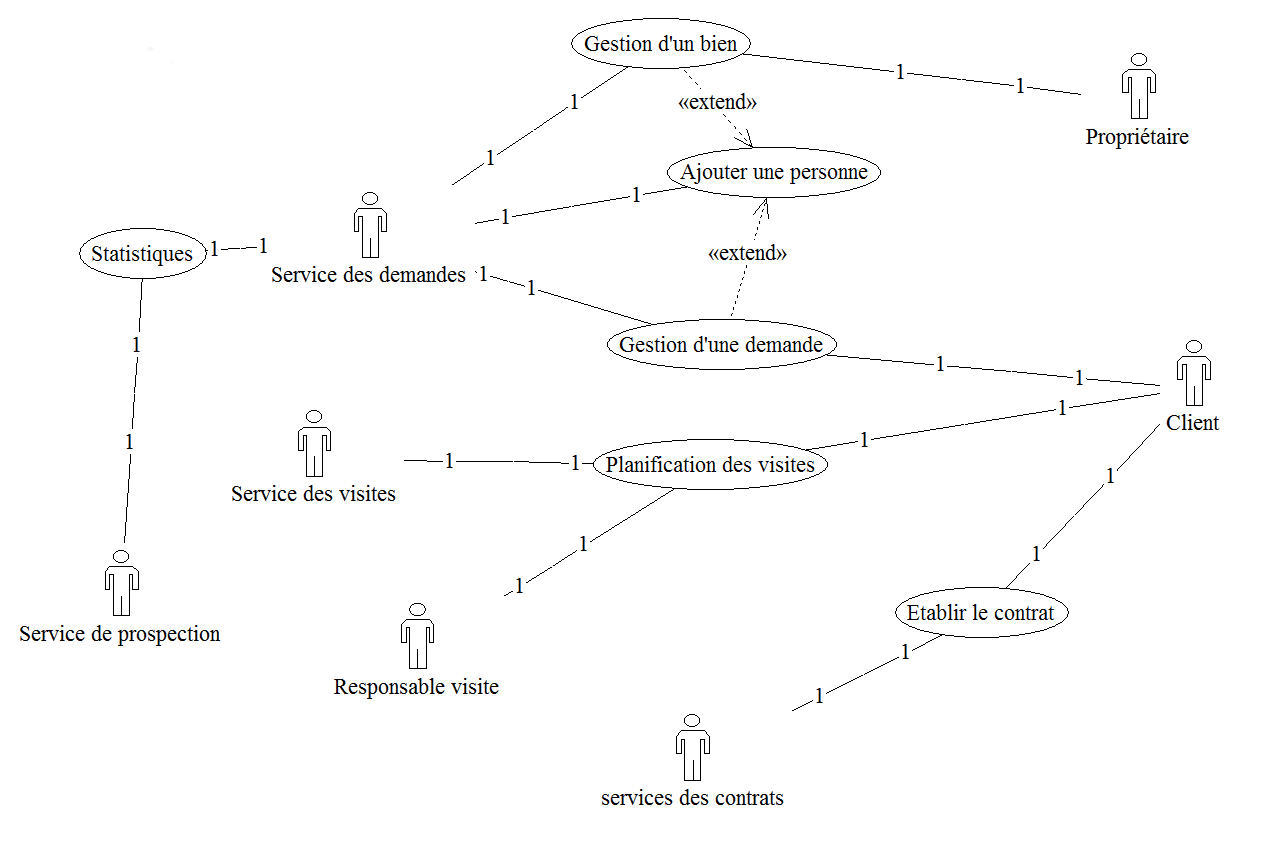
\includegraphics[width=16cm]{use-case.png}
\caption{Use-case diagram, réalisé à l'aide de DB-Main}
\label{fig:diagUC}
\end{figure}

\newpage
\subsection{Activities}
A l'aide des scénarios établis lors de l'étape précédente, nous avons pu établir des diagrammes d'activités. Ces diagrammes ont pour but de modéliser les flux d'informations entre l'acteur impliqué dans le scénario et le système.
Ce diagramme nous sert pour visualiser de manière plus claire, notamment les conditions qui peuvent être rencontrées au cours d'une action.\\

Dans le cas présent, nous avons réalisé ces diagrammes afin de nous conforter dans ce que les use-case nous ont apporté, et éventuellement les compléter, car ils sont forts liés l'un à l'autre. Ceci nous a confirmé les choix effectués lors de l'établissement du schéma entité-association.

\subsubsection{L'ajout d'une personne}
\begin{figure}[H]
\centering
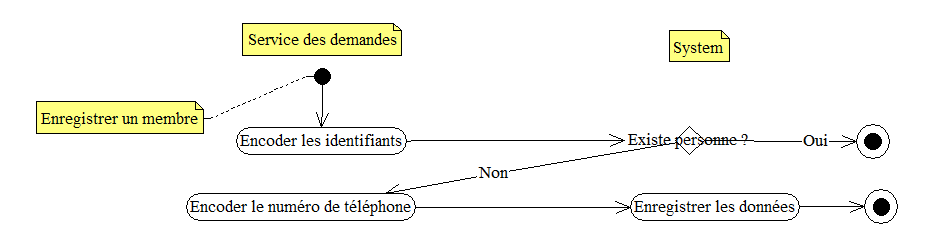
\includegraphics[width=16cm]{ajoutMembre.png}
\caption{Activity diagram de l'ajout d'une personne dans le système.}
\label{fig:ajoutMembre}
\end{figure}

Note : les identifiants de vérification  de l'unicité sont, comme mentionné dans le scénario, le nom, le prénom, et l'adresse.

\subsubsection{L'ajout d'un bien}
\begin{figure}[H]
\centering
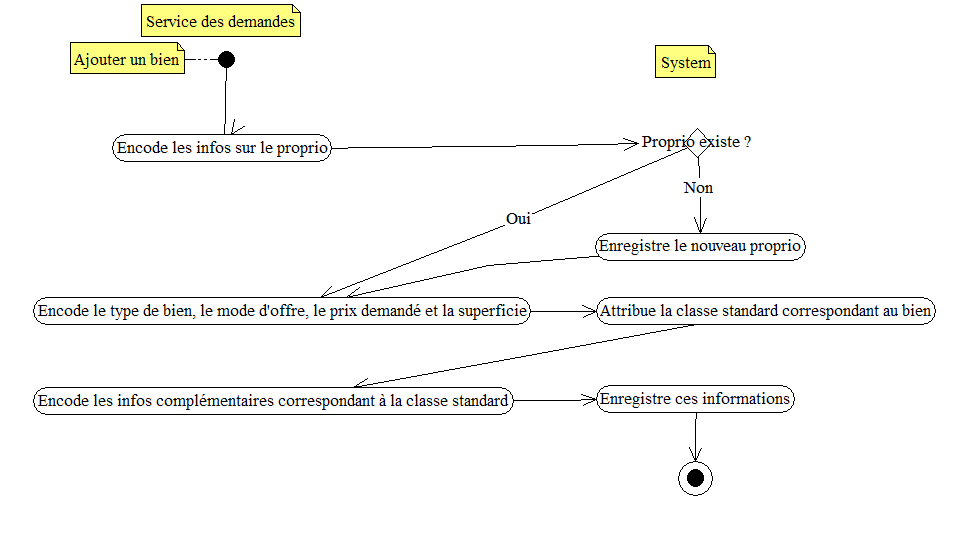
\includegraphics[width=16cm]{ajoutBien.png}
\caption{Activity diagram de l'ajout d'un bien dans le système.}
\label{fig:ajoutBien}
\end{figure}
Dans le cas présent, nous voyons clairement l'interaction de cette fonctionnalité, qui dans son mode de fonctionnement, intègre la fonctionnalité d'ajout d'un membre.

\subsubsection{La gestion de la demande d'un client}
\begin{figure}[H]
\centering
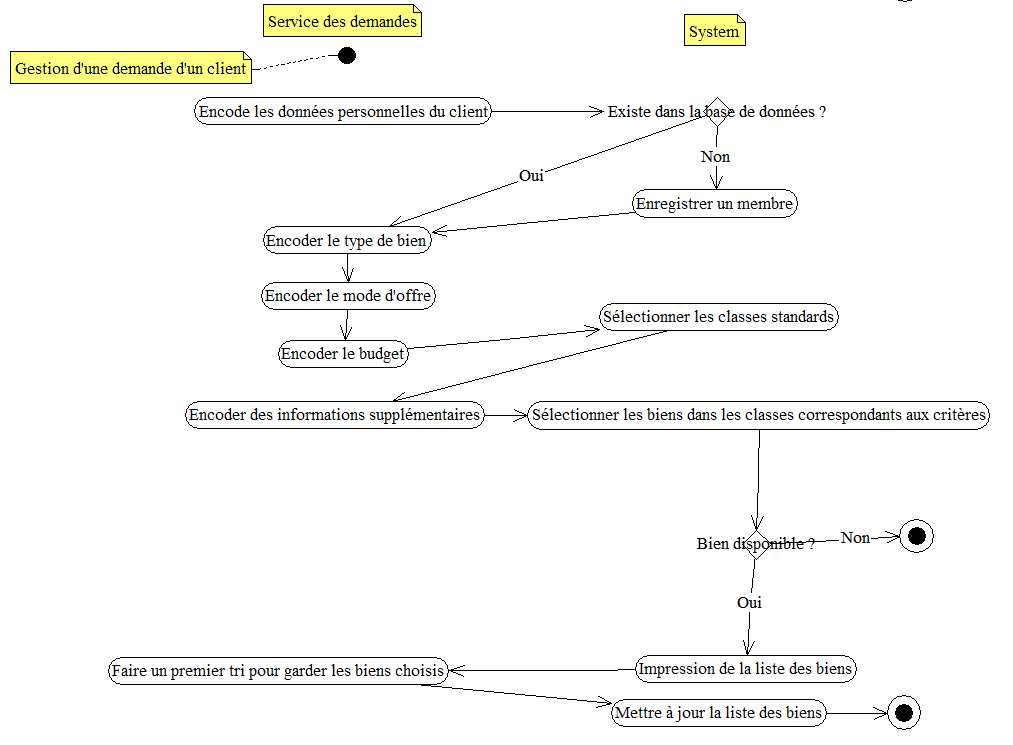
\includegraphics[width=16cm]{demandeBien.png}
\caption{Activity diagram de la demande d'un bien par un client.}
\label{fig:demandeBien}
\end{figure}
Comme dans pour le schéma d'ajout d'un bien dans le système, on voit ici clairement l'interaction entre fonctionnalités.

\subsubsection{La planification des visites}
\begin{figure}[H]
\centering
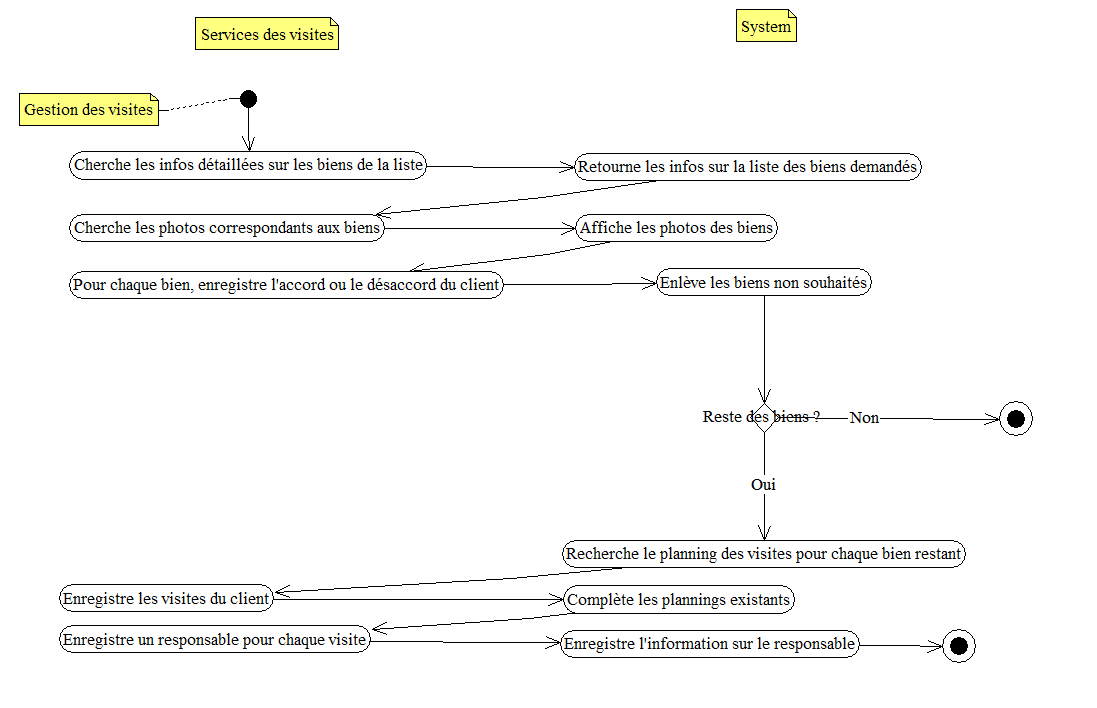
\includegraphics[width=16cm]{visites.png}
\caption{Activity diagram de l'organisation des visites.}
\label{fig:visites}
\end{figure}

\subsubsection{L'établissement d'un contrat}
\begin{figure}[H]
\centering
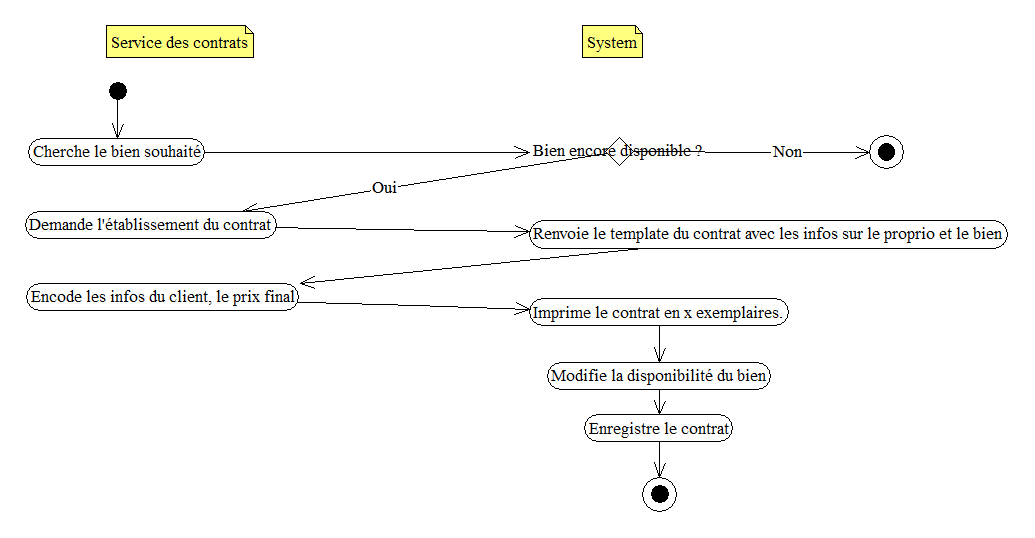
\includegraphics[width=16cm]{contrat.png}
\caption{Activity diagram de l'établissement d'un contrat.}
\label{fig:contrat}
\end{figure}

\subsubsection{La création des statistiques}
\begin{figure}[H]
\centering
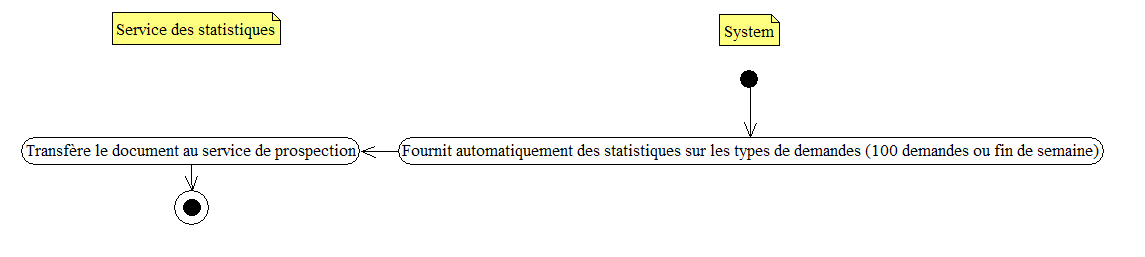
\includegraphics[width=16cm]{stats.png}
\caption{Activity diagram de la génération des statistiques.}
\label{fig:stats}
\end{figure}
\mbox{}
\subsection{Modélisation UML}
A partir de l'analyse initiale ainsi qu'avec les informations obtenues à l'aide du diagramme des use-case et du diagramme des activities, nous avons pu établir un premier diagramme de classe. Ce diagramme de classe, aussi appelé UML, représente un schéma des différentes entités (futurs tables) principales que nous allons retrouver plus tard dans la base de données. Nous pouvons aussi y trouver les associations nommées entre ces entités, et les cardinalités associées. Le logiciel que nous avons utilisé ne nous permettant pas d'autres cardinalités que 1 ou *, 1 vaut pour 1-1 et 0-1, tandis que * vaut pour 1-N et 0-N.\\

Le diagramme UML nous permet également de visualiser les fonctions nécessaires au bon fonctionnement du système d'informations. Dans le cas du diagramme que nous présentons à la page suivante, les fonctions définies sont les premières auxquelles nous avons pensé. Nous aurions du compléter ce diagramme à l'aide des fonctionnalités découvertes à l'aide des diagrammes de séquences, définis à la prochaine section. Cependant, nous avons manqué de temps, et nous n'avons pas su terminer les diagrammes de séquence. De ce fait, nous avons délibérément choisi de montrer le diagramme UML défini auparavant, ceci pour éviter d'avoir quelque chose de mal balancé dans nos classes.


\newpage
\begin{landscape}
\begin{figure}[H]
\centering
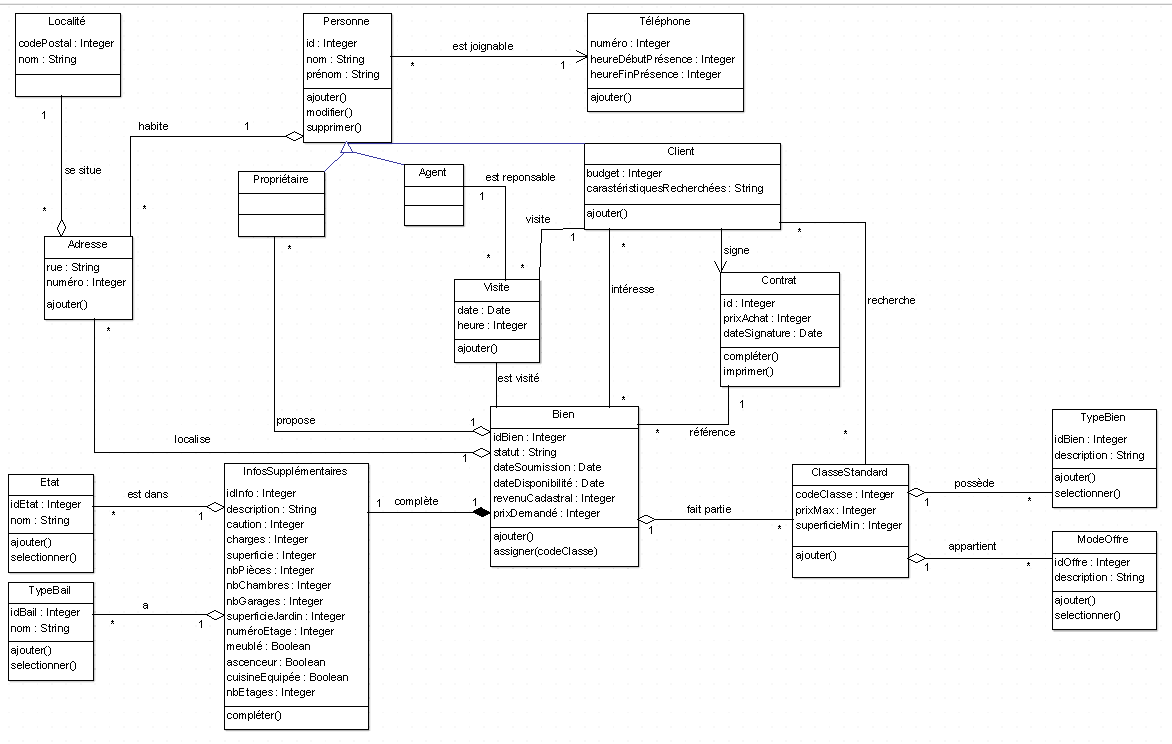
\includegraphics[width=23cm]{uml.png}
\caption{UML sur base des résultat des analyses précédentes.}
\label{fig:uml}
\end{figure}
\end{landscape}
\subsection{Diagramme de séquence}
Le diagramme de séquence a pour objectif de montrer les interactions entre les classes du diagrammes UML selon un use-case.
Nous présentons uniquement notre diagramme de séquence pour la gestion d'une demande.
Nous n'avons pas eu le temps de faire les autres use-cases.

\subsubsection{La gestion d'une demande}
L'acteur principal est le service des demandes. 
Il commence par vérifier l'existence du client via l'opération \texttt{checkExistence()}.
Cette opération prend le nom, le prénom et l'adresse en entrée et renvoie un booléen.
Ce booléen permet alors soit de continuer les opérations, soit de créer un nouveau Client.
Le nouveau Client est crée via la méthode \texttt{new()} de Personne.
Par la suite, le service enregistre le mode d'offre, le type de bien et le budget du client.
Ces informations sont sauvegardées par l'opération \texttt{savePreference()}.
Suite à cela, le système va chercher les classes standards respectant les critères du client via l'opération \texttt{getAllClasseStd()}.
L'employé ajoute les informations supplémentaires avec l'opération \texttt{saveInfosComplementaire()}.
Ces informations regroupent le choix du client sur plusieurs critères (présence d'un jardin, nombre de chambres, etc.).
L'opération \texttt{getListeBiens()} enregistre pour un client, selon ces critères et les classes standards qui lui sont associées, les biens disponibles.
Finalement, l'opération \texttt{updateList()} sert à peaufiner la liste générée à l'étape précédente.
Ce tri est dicté par le client sur ses premières impressions.\\

Un schéma représentant les interactions entre les classes est disponible à la figure \ref{fig:sequence} p.\pageref{fig:sequence}

\newpage
\begin{landscape}
	\begin{figure}
		\centering
		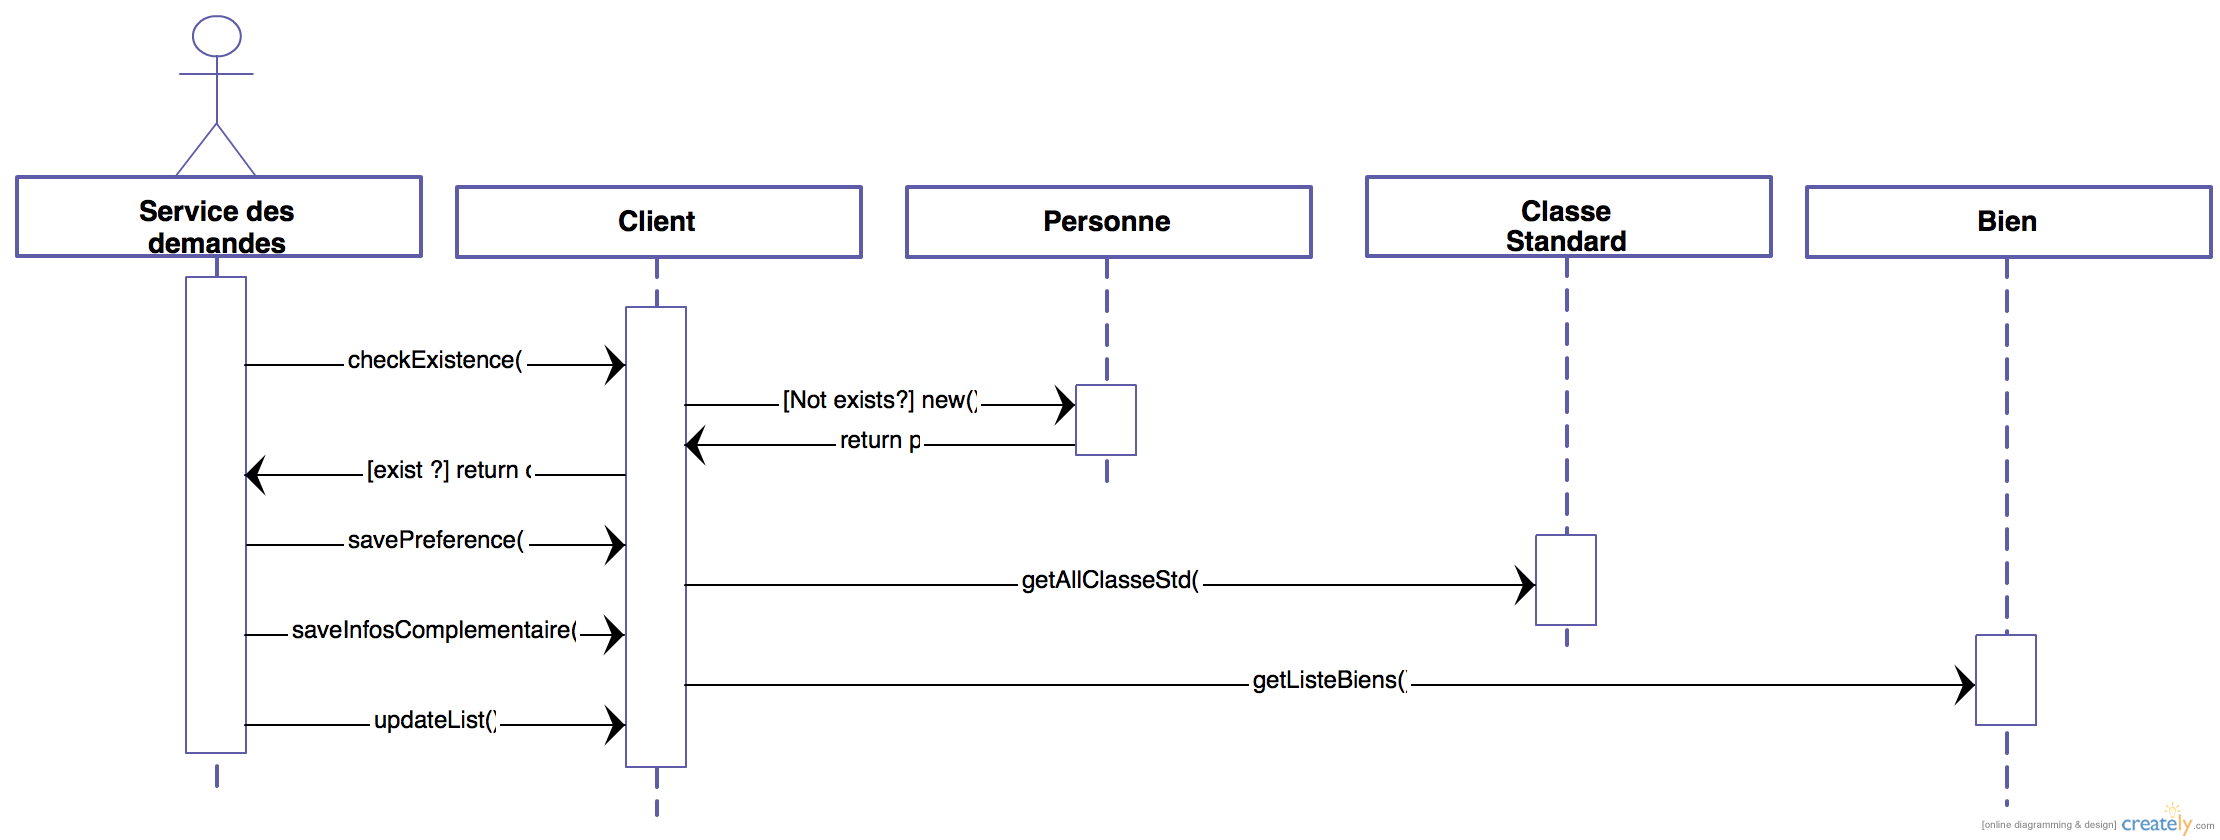
\includegraphics[width=23cm]{Sequence-DemandeBien.png}
		\caption{Diagramme de séquence - Gestion d'une demande}
		\label{fig:sequence}
	\end{figure}	 
\end{landscape}
\newpage
\mbox{}
\thispagestyle{empty}
\newpage
\section{Description de la base de données}
Cette partie du rapport est destinée à la description de notre base de données. Celle-ci se base sur les différentes analyse que nous avons précédemment décrites dans ce cahier des charges. Ci-dessous se trouvent les schéma entité-association ainsi que le schéma relationnel qui en découle.

\subsection{Schéma entité-association}
Le schéma entité-association représente, comme son nom l'indique, les entités composant la base de données ainsi que les associations qui relient celles-ci. Afin de composer ce schéma final, nous avons repris celui que nous avons décrit lors de la première analyse du cas. Nous avons par la suite ajouté ce que nous avons pu remarquer comme éléments supplémentaires à l'aide des use-case, activities, et diagramme UML. Nous n'avons pas pris en compte le diagramme séquentiel et les champs supplémentaires qu'il apportait, pour les raisons qui ont été mentionnées dans les sections précédentes.\\

Le schéma entité-association créé dans DB-Main est représenté par la figure \ref{fig:ea}, à la page \pageref{fig:ea}.

\subsection{Schéma relationnel}
Le schéma relationnel découle du schéma entité-association. Il s'agit de la représentation de celui-ci sous forme de tables afin de constituer la base de données voulue. Les associations sont donc transformées soit en tables soit en clé étrangère selon la cardinalité des associations précédentes.\\

Comme vu dans le schéma entité-association (fig.~\ref{fig:ea} p.\pageref{fig:ea}), les entités \textit{client}, \textit{propriétaires}, \textit{agent} sont de spécialisations de l'entité \textit{personne}. Nous avions donc le choix pour le représentation relationnelle entre combiner ces trois entités spécialisées dans une même table ou de les dissocier dans trois tables. Nous avons opté pour la deuxième solution. En effet, il est plus aisé d'avoir les clients séparés des agents et des propriétaires dans des tables distinctes, car ces entités ont des attributs différents. Nous avons plus d'informations à conserver pour un client que pour un propriétaire.\\

Le schéma de la base de données est la figure \ref{fig:bdd} à la page \pageref{fig:bdd}.
Le présent schéma a été généré à partir de notre schéma entité-association dans DB-Main.





\newpage
\begin{landscape}
	\begin{figure}
		\centering
		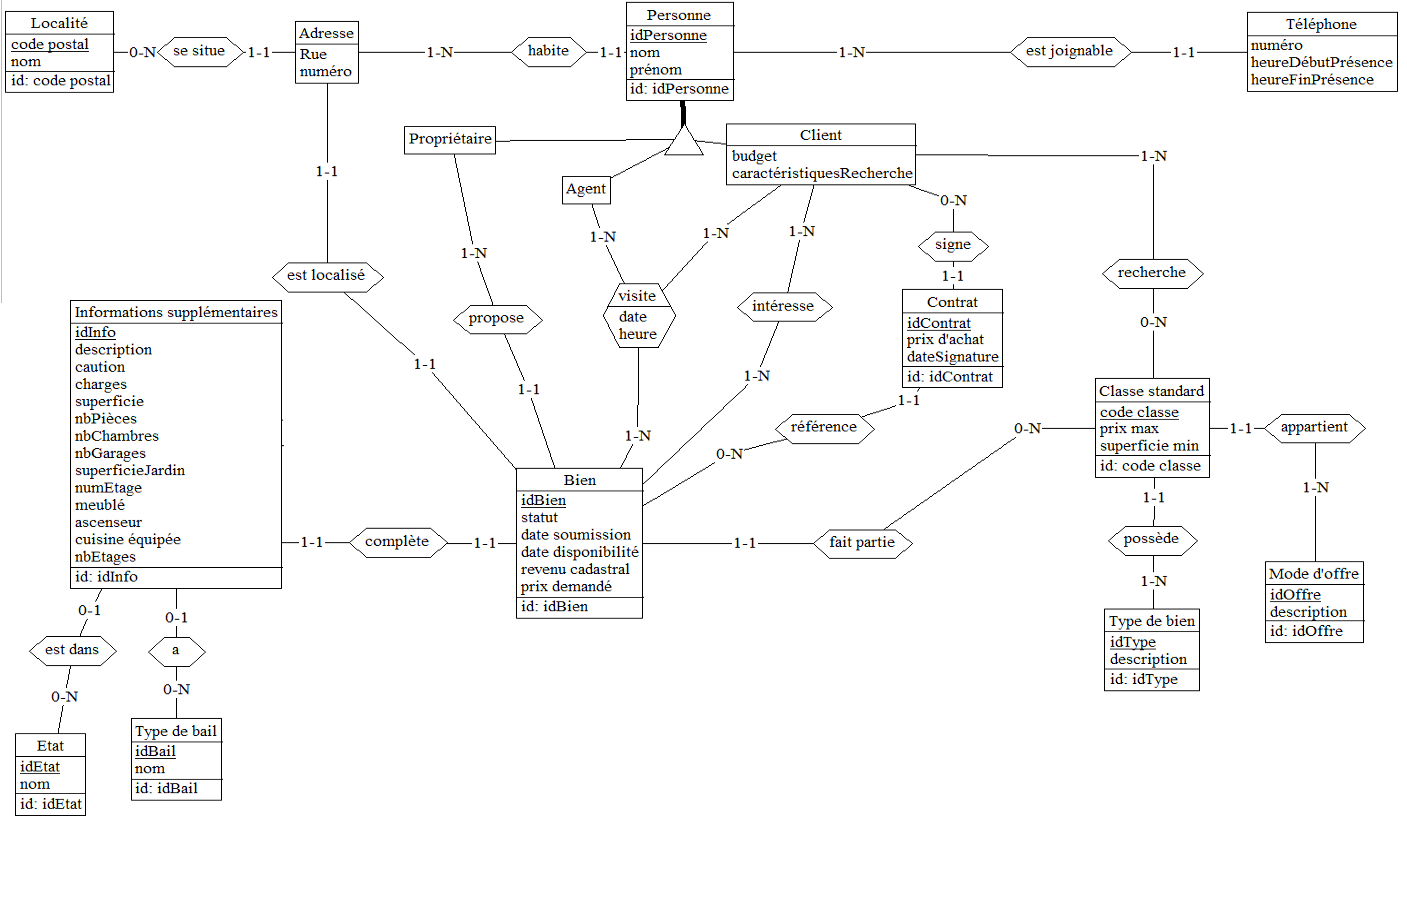
\includegraphics[width=25cm]{association.png}
		\caption{Schéma entité-association final}
		\label{fig:ea}
	\end{figure}
\end{landscape}

\begin{figure}[H]
	\centering
	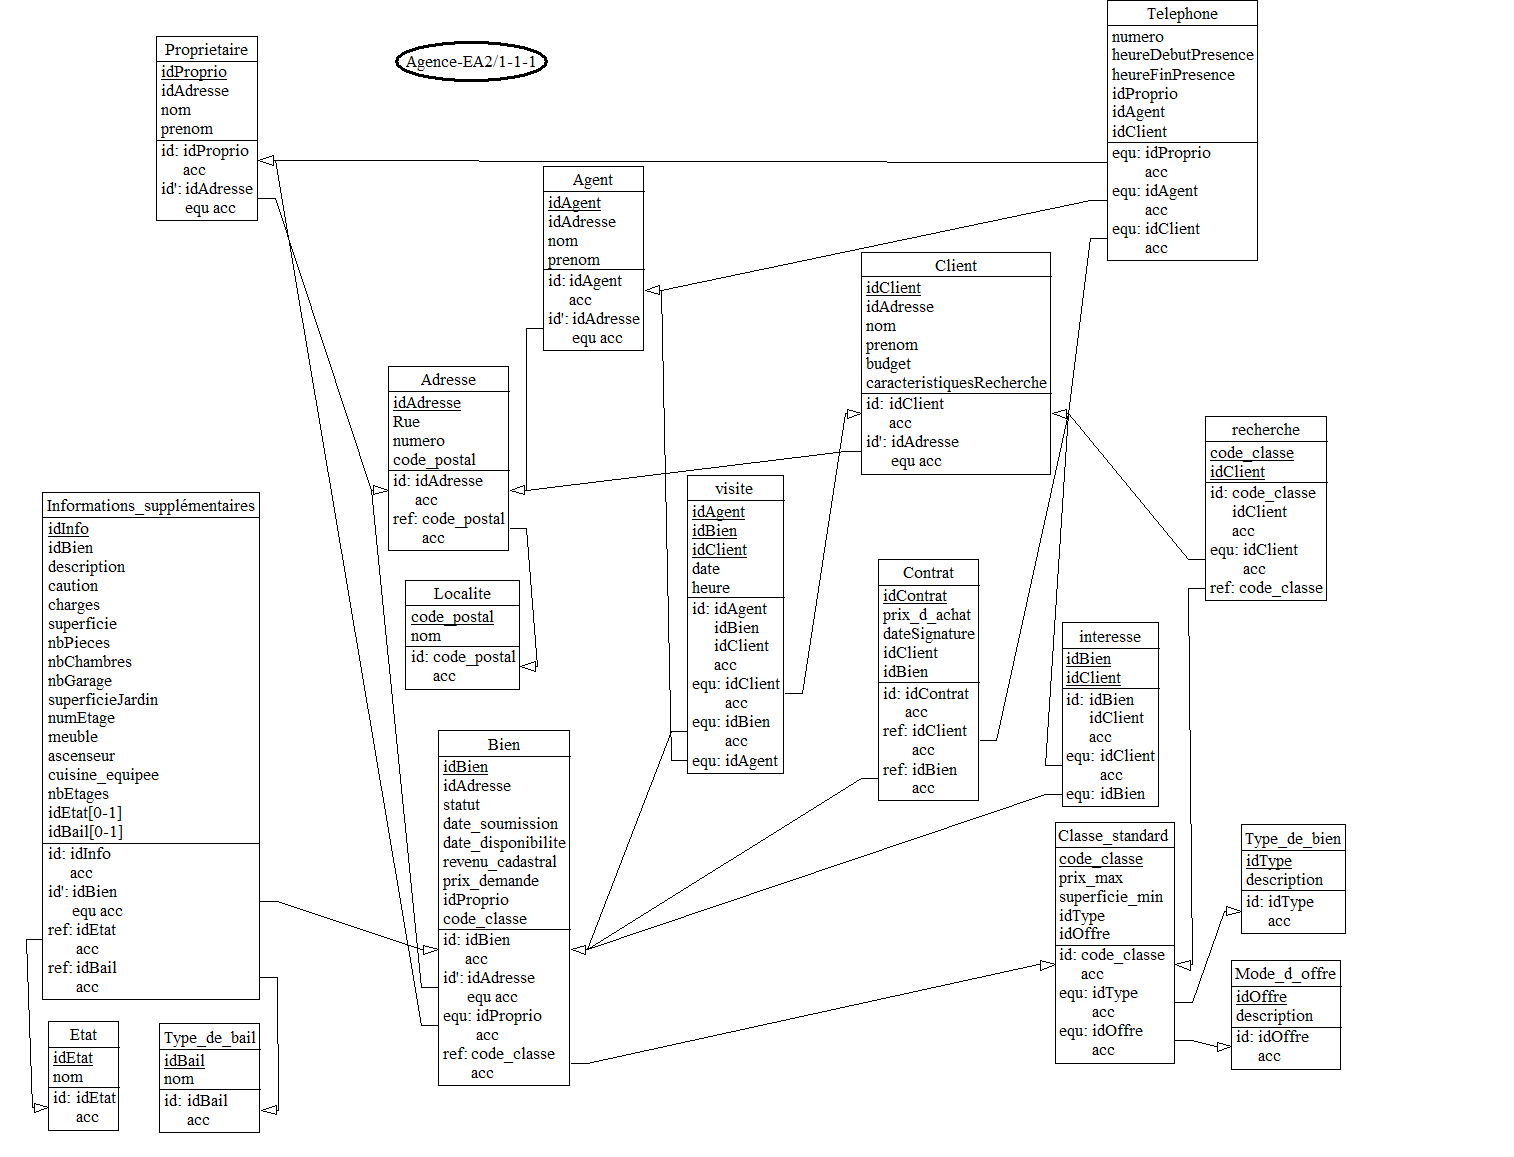
\includegraphics[width=16cm]{relationnel.png}
	\caption{Schéma de la base de données}
	\label{fig:bdd}
\end{figure}


\newpage
\mbox{}
\thispagestyle{empty}
\newpage
\newpage
\section{Conclusion}
Au terme de ce cahier des charges, nous pensons avoir fourni une solution viable et correcte afin de répondre aux besoins de système d'informations de l'agence immobilière.\\

Nous avons commencé par réaliser une première analyse des documents fournis par l'agence, afin d'en tirer une ébauche de schéma entité-association. Cette ébauche a par la suite été complétée à l'aide de différents outils. Nous nous sommes servis des diagramme de type use-case afin de définir les grandes fonctionnalités du système. Nous en avons élaboré les scénarios complets afin de vérifier la justesse de notre schéma entité-association et le corriger si nécessaire. Par la suite, nous avons traduit ces scénarios en diagrammes d'activité, représentant les interactions entre les acteurs des scénarios, le système, et les conditions rencontrées en cours de traitement. Nos avons enfin complété notre ébauche à l'aide des diagrammes UML. Nous aurions aimé rendre nos entités encore plus précises à l'aide des diagramme de séquence, mais nous avons manqué de temps pour l'élaboration de ceux-ci. Nous nous sommes donc contentés de ce qui avait été réalisé auparavant.\\

Au final, nous sommes arrivés a un schéma entité-association complété par les différents outils mis à notre disposition, réalisé sous DB-Main. Ce schéma association répond aux attentes de l'agence immobilière pour la réalisation de leur système d'informations. Ce schéma final a enfin été traduit en schéma relationnel. Celui-ci représente la base de données à implémenter pour l'agence immobilière, sous forme des diverses tables, ainsi que les tables ajoutées par les associations, les clés primaires, et les clés étrangères liant le tout.\\

Nous espérons, au travers de ce document, avoir répondu à la demande de système d'informations de la part de l'agence immobilière. Nous osons croire que l'analyse que nous avons fournie est suffisamment complète et satisfera notre client.
\newpage
\mbox{}
\thispagestyle{empty}
\newpage
\newpage
\section*{Ressources utilisées}
\addcontentsline{toc}{section}{\protect\numberline{}Ressources utilisées}
\begin{enumerate}
\item FAULKNER Stéphane, slides utilisées dans le cadre du cours d'\textit{Architecture base de données} des 3TI, Ephec, 2014-2015.
\item DB-Main, logiciel de modélisation de bases de données, \url{http://www.db-main.be/}
\item ArgoUML, UML Modeling Tool, \url{http://sourceforge.net/projects/argouml.mirror/}
\item Creately,  Online Diagram Software to draw Flowcharts, UML, ..., \url{http://creately.com/}
\end{enumerate}


\end{document}